%\documentclass[10pt,twocolumn]{IEEEtran}
% to specify a filename, can use:
\documentclass[10pt,twocolumn]{IEEEtran}
%\usepackage{epsfig}
\usepackage{graphicx}

% I didn't like list-s
\hyphenation{lists}
\pagestyle{empty}

% We need to obtain a command to tell us if a command has
% been previously defined so that we can determine which
% IEEEtran.cls is running. The \makeatletter stuff provides
% a way to "get at" the internal command \@ifundefined
% since it contains the @ character
\makeatletter
\def\ifundefined{\@ifundefined}
\makeatother

% V1.1 change: The font change commands have to be located
% in the preamble before the title or author is declared.
% If you uncomment these, you may also want to uncomment
% the redefinition of \PARstart around line 258 so that
% the big first letter is in the same font as the rest of
% the text.
% Here is how you can go back to the Computer Modern fonts
% if you wish:
%\renewcommand{\sfdefault}{cmss}
%\renewcommand{\rmdefault}{cmr}
%\renewcommand{\ttdefault}{cmtt}

%\usepackage{hrefpdf}

\begin{document}


\title{\LARGE \bf LeVinQam: A Question Answering Mining platform}

\author{
\large Patrick Duval, Agathe Merceron, Christian Rinderknecht, Michel Scholl \\ 
\normalsize ESILV - G\'enie Informatique\\ 
\normalsize P\^ole Universitaire L\'eonard de Vinci\\ 
\normalsize F-92916 Paris La D\'efense - Cedex \\
\normalsize FRANCE \\ 
\normalsize {\it \{patrick.duval, agathe.merceron, christian.rinderknecht, michel.scholl\}@devinci.fr}
}

% The major version number of the class file will not
% be defined with the old IEEEtran.cls. So, we can use this fact
% to determine if we are running the old or the new class.
\ifundefined{IEEEtransversionmajor}{%
   % This block will be executed only if we are using the old
   % class. All we do is to make sure the V1.3 lengths and commands
   % actually exist so the code won't choke when it
   % doesn't find them.

   % This file doesn't need most of these definitions.
   % However, we'll provide them all in case somebody
   % wants to see what should be executed when compiling
   % a V1.3 or later IEEEtran.cls .tex file with a pre V1.3
   % IEEEtran.cls class file. In such a case, all you have to
   % do is copy this block to the start of your code.
   % However, it won't fix any bugs in the old IEEEtran.cls!
   %
   % **** BACKWARD COMPATIBILITY CODE BLOCK START ****
   \newlength{\IEEEilabelindent} \newlength{\IEEEilabelindentA}
   \newlength{\IEEEilabelindentB} \newlength{\IEEEelabelindent}
   \newlength{\IEEEdlabelindent} \newlength{\labelindent}
   \newlength{\IEEEiednormlabelsep} \newlength{\IEEEiedmathlabelsep}
   \newlength{\IEEEiedtopsep}

   \providecommand{\IEEElabelindentfactori}{1.0}
   \providecommand{\IEEElabelindentfactorii}{0.75}
   \providecommand{\IEEElabelindentfactoriii}{0.0}
   \providecommand{\IEEElabelindentfactoriv}{0.0}
   \providecommand{\IEEElabelindentfactorv}{0.0}
   \providecommand{\IEEElabelindentfactorvi}{0.0}
   \providecommand{\labelindentfactor}{1.0}

   \providecommand{\iedlistdecl}{\relax}
   \providecommand{\calcleftmargin}[1]{ \setlength{\leftmargin}{#1}
   \addtolength{\leftmargin}{\labelwidth}
   \addtolength{\leftmargin}{\labelsep}}
   \providecommand{\setlabelwidth}[1]{ \settowidth{\labelwidth}{#1}}
   \providecommand{\usemathlabelsep}{\relax}
   \providecommand{\iedlabeljustifyl}{\relax}
   \providecommand{\iedlabeljustifyc}{\relax}
   \providecommand{\iedlabeljustifyr}{\relax}

   \newif\ifnocalcleftmargin \nocalcleftmarginfalse

   \newif\ifnolabelindentfactor \nolabelindentfactorfalse

   % in V1.4 of IEEEtran.cls 
   \newif\ifcenterfigcaptions
   \centerfigcaptionsfalse

   % we need to provide the old IED environments 
   % with a bogus optional argument 
   \let\OLDitemize\itemize
   \let\OLDenumerate\enumerate \let\OLDdescription\description

   \renewcommand{\itemize}[1][\relax]{\OLDitemize}
   \renewcommand{\enumerate}[1][\relax]{\OLDenumerate}
   \renewcommand{\description}[1][\relax]{\OLDdescription}

   \providecommand{\pubid}[1]{\relax}
   \providecommand{\pubidadjcol}{\relax}
   \providecommand{\specialpapernotice}[1]{\relax}
   \providecommand{\overrideIEEEmargins}{\relax}

   % V1.1 change: use \let instead of \providecommand % This prevents
   %LaTeX from hanging if the user ever % tried to redefine \PARstart
   %in terms of \CMPARstart 
   \let\CMPARstart\PARstart

   \let\OLDappendix\appendix
   \renewcommand{\appendix}[1][\relax]{\OLDappendix}

   \newif\ifuseRomanappendices 
   \useRomanappendicestrue

   % V1.2 change: handle the optional biography environment argument %
   %(the photo specifier) provided by IEEEtran V1.5 and later.  % This
   %is tricky because, under the new biography, the SECOND % argument
  % is the non-optional one (the biography text).
   \let\OLDbiography\biography 
   \let\OLDendbiography\endbiography
   \renewcommand{\biography}[2][\relax]{\OLDbiography{#2}}
   \renewcommand{\endbiography}{\OLDendbiography} 
   % **** BACKWARD COMPATIBILITY CODE BLOCK END ****

    % alter the header to show we are using the older class
   %\markboth{A Test for IEEEtran.cls--- {\tiny \bfseries
   %[Running Older Class]}}{Shell: A Test for IEEEtran.cls}}{
   % END IF OLDER CLASS

   % This block will be executed only if we are running
   % the enhanced class
   % alter the header to show we are using the enhanced class
   \markboth{A Test for IEEEtran.cls--- {\tiny \bfseries [Running
   Enhanced Class V\IEEEtransversionmajor.\IEEEtransversionminor]}}%
   {Shell: A Test for IEEEtran.cls}}
% end of conditional


% Uncomment this line to render the big first letter in
% Computer Modern font.
%\renewcommand{\PARstart}[2]{\CMPARstart{#1}{#2}}
% V1.1 change: This would hang if using the older IEEEtran.cls
% in IEEEtest V1.0, it is OK now.
%
%
% Here's how you would do invited papers:
%\specialpapernotice{(Invited Paper)}
% If you are binding copies of work generated with IEEEtran.cls,
% you may want to try:
%\overrideIEEEmargins
% These commands work OK here even though they are not in the preamble.
%(I wanted to put them after the backward compatibility code)


\maketitle
\thispagestyle{empty}
% here's how you get a publisher's ID mark with the new
% IEEEtran.cls.  If you want to use it, don't forget to
% also uncomment the \pubidadjcol command (which must be
% executed in the second text column) around line 434 below
%\pubid{0000--0000/00\$00.00~\copyright~2001 IEEE}


%\begin{abstract}
 
%MS � am�liorer
The development of Web technologies has accelerated the offer of
(commercial) e-learning platforms. 
This paper is a first step toward the design and implementation of a
platform called LeVinQam whose main functionalities are (a) the provision and
management of a series of exercises and tests (authoring tools), (b) a
personalized navigation through the 
existing collection  of  exercises and tests, taking into account the
user profile (level of skills) and history, (c) the analysis of user
answers, its storing into a 
database and its mining. 
As   case studies  we have  chosen (1) the
learning of SQL, the standard database query language, and (2) formal proofs for propositional logic, to validate the 
platform functionalities  and the mining of answers.




% no need for this single page document
% you may have to move \pubidadjcol (if used) if
% these are enabled
%\listoffigures
%\listoftables
%\tableofcontents

\section{Introduction} %MS
\label{intro}
%%-*-latex-*-

\section{Introduction}

The wide variety of software and hardware architectures in distributed
systems and telecommunications makes it valuable to use a common
high-level data notation in protocol specifications. To fulfill this
need, the ISO organization and the International Telecommunication
Union (ITU) defined the Abstract Syntax Notation One (\ASN) series of
standards. \ASN~\cite{Dubuisson:2000,X.680:2002,X.681:2002,X.682:2002,X.683:2002}
is a language for data types allowing the protocol designer to capture
numerous networking concepts, such as protocol data units, without
worrying about the possible environment and implementation
heterogeneity of the peers. The peers share a set of \ASN modules and
agree upon a set of \emph{encoding rules}, such
as~\cite{X.690:2002,X.691:2002}, which is a method for encoding values
produced at run-time by the communicating applications, into series of
bits. \ASN has been adopted for a wide range of applications, such as
network management, secure e-mail, mobile telephony, air traffic
control etc.
%, video conferencing over the internet, electronic commerce,
%digital certificates, radio paging, financial service systems etc.

\medskip

In the last few years, the press has reported several alleged
vulnerabilities of \ASN and the Basic Encoding Rules (BER) related to
network protocols like SNMP and, more recently, OpenSSL. Each time, an
accurate description of the problem has been finally published,
showing that the weakness lay in \emph{implementations} poorly written
and insufficiently tested. The real vulnerabilities were almost all
related to improper decoding of ill-formed BER encodings (or
\emph{codes}) causing buffer overflows, unspecified
(non-deterministic) behaviours, stack corruptions and, in the end, a
possible denial of service.

\medskip

From now on, it is important to understand and remember that \ASN and
the BER, intrinsically, have nothing to do with security or
cryptographic protocols. Both are used for modeling and handling the
data part of protocols, not the control. As a consequence, the
soundness property we aim at in this article must not be considered as
a security property about \emph{control} but as mere correctness of
composition of encoding and decoding with the BER of \emph{values}
specified by means of \ASN. For instance, there are no attackers, no
nonces etc. here. Nevertheless, the difficulty is not lesser.

\medskip

More precisely, in this work we want to prove that the design of the
BER themselves is flawless, whatever the network protocol is and
whatever the values to be transmitted are. To achieve this goal we
need the support of formal methods. We start by a formal modeling of
the BER which abstracts away low-level details but captures the design
principles. Then we define a soundness property representing the
security warranty we require and finally we prove that this property
holds for all values that can be specified with \ASN.




\section{e-Learning Information Model} %MS
\label{model}
%%-*-latex-*-

\section{Formal model}
\label{model}

A formal model is a framework based on logic that allows one to define
precisely the concepts involved in a problem and its solution. In
order to reduce the gap between the program and its specification, we
restrict ourselves to basic mathematical constructs that can be mapped
to data structures and functions of the implementation programming
language. Functions here are elementary functions over sets of
objects, called \emph{terms}, so the implementer can translate them
into functions, procedures, methods, processes etc., depending on the
target. Let us review the different kinds of terms in our formal
model.
\begin{itemize}

  \item \emph{Integers} are the familiar numbers.

  \item \emph{Variables} are names, e.g., \(x\), \(y\) or \(z\). We
    assume that there exists a denumerable infinity of them.

  \item \emph{Tuples} are finite and ordered sets of terms.  Each term
    in a tuple is called a \emph{component}. Tuples can be nested, as
    in \((a, (b, c), d)\).  The empty tuple is \(()\).

  \item \emph{Lists} are possibly empty series of terms, called
    \emph{items}. The first item is called the \emph{head} and the
    remaining sub\hyp{}list the \emph{tail}. Here, we shall follow the
    \Prolog notation for lists and write \(\el\) for the empty list
    and \(\cons{e}{l}\) for the non\hyp{}empty list whose head is
    (denoted by) \(e\) and tail is (denoted by) \(l\). Some shorthands
    prove useful, like writing \([a, b, c]\) instead of
    \(\cons{a}{\cons{b}{\cons{c}{\el}}}\). It is also convenient
    sometimes to distinguish several items past the head, and write
    \(\cons{a, b}{l}\) instead of \(\cons{a}{\cons{b}{l}}\).  Notice
    also that, from an algorithmic point of view, the lists of our
    model are \emph{stacks} (the head of the list corresponds to the
    top of the stack).
%% From an implementation point
%%    of view, e.g., in \Clang, lists can be one\hyp{}way linked lists.

  \item \emph{Constructors} are names which can be associated with a
    tuple of terms. They act like a tag for a tuple and, as such, are
    always written with the tuple they distinguish (the constructor
    precedes the tuple).  For example \(c(1, d(n))\) is a term
    constructed with constructors \(c\) and \(d\). It is possible for
    the tuple to be empty. 
%% (In \Clang, this situation corresponds to enumerated values.)  
    For example, \(c(1, d())\) contains the
    constructor \(d\) applied to (that is, tagging) the empty tuple.
    Note that, in order to distinguish constructors from variables, we
    always retain the parentheses, like \(d()\) (whereas \(d\) alone
    is a variable). The number of components of a constructor \(c\) is
    called \emph{arity} and noted \(A(c)\).

%Different tuples tagged by the same constructor are supposed to belong
%to the same set of constructed terms.

\end{itemize}
\piccaption{\label{tree}}
\smallskip
\parpic[r]{\fbox{\includegraphics[bb=72 652 123 721]{tree}}} It is
useful to graphically represent terms as \emph{trees}. Constructors
then denote \emph{nodes} and their components denote subtrees. Empty
tuples, variables and integers denote \emph{leaves}. For example
\(d((), e([1]))\) can be interpreted as a tree of \emph{root} \(d\)
and whose first subtree is the representation of the empty tuple
\(()\) and the second corresponds to \(e([1])\). Figure~\ref{tree}
represents the tree corresponding to \(a(b(c(1), (\el, 2)), (),
d(d(x)))\), where the root is \(a\) and the leaves are \(1\), \(\el\),
\(2\), \(()\) and \(x\). When a tuple has no constructor, the
corresponding inner node is a centered dot. Arity is constant for each
kind of node, so we cannot have in the model both \(c(a())\) and
\(c(a(),b())\). In other words, our trees are \emph{ranked}. Never the
less, for technical reasons, it is useful to have unranked trees. The
way to circumvent this limitation is to encode a variable arity by an
arity of \(1\) and a list as subtree. Then we can have both \(c([1])\)
and \(c([1, (2)])\) and pretend that the arity of \(c\) is \(1\) in
the former case and \(2\) in the latter.

Let us now use these generic terms to build the terms that model the
problem at hand.

\paragraph{Lexemes.}

The first stage of a compiler consists in the lexical analysis
(sometimes called scanning or lexing) of the source code: the input
string of characters is analysed and segmented into the longest
substrings that can be classified according to the lexicon of the
input language. This is similar to transforming a line of text into
words that have been checked against a dictionary. The output consists
of a series of \emph{lexemes}. Since the ambition of this study is to
cope with all programming languages, we shall make no assumptions on
the nature of the lexemes. We shall often designate a lexeme by \(l\)
and their (unspecified) set will be noted \(\cal L\).

\paragraph{Concrete\hyp{}Syntax versus Abstract\hyp{}Syntax Trees.}

The second stage of a compiler is the syntax analysis, also known as
\emph{parsing}, of the lexeme stream. This is akin to checking whether
a series of words makes up a correct sentence, with respect to a given
grammar, like the English grammar. The result of such a process is a
tree called the \emph{concrete\hyp{}syntax tree}, or \emph{parse
tree}, capturing the structure of the analysed sentence in terms of
the language grammar. In practice, this tree is usually not built
entirely and lives in the analysis stack of the parser for the time of
the processing. Instead, the programmer often chooses to output a
tree, called \emph{abstract\hyp{}syntax tree} (AST), which also
captures the structure of the input program, with or without
references to the grammatical rules. The inner nodes of the parse tree
denote non\hyp{}terminal symbols of the grammar, as usually specified
in Backus\hyp{}Naur Form or an extended version of it, and the leaves
are the lexemes of the input. In contrast, the AST usually does not
include the lexemes (see our example in the introduction) and the
nodes denote kinds of constructs with or without reference to the
grammar. Therefore, the converse of parsing, called \emph{unparsing},
is naturally defined on the parse tree. On the one hand, the parse
tree is not available as a data structure and, on the other hand, the
AST can be arbitrary. Fortunately, the AST is often quasi isomorphic
to the parse tree or is a compact version of it, which makes unparsing
from the AST workable in practice. Therefore, without loss of
generality, we define the unparsing inductively on the structure of
the parse tree, which renders the unparsing dependent only on the
grammar.

Each non\hyp{}terminal symbol of the grammar corresponds to one or
more constructors of the parse tree, depending on the number of
productions with that symbol on the left\hyp{}hand side. For example,
the productions \verb/Exp ::= Integer | Exp + Exp/ \verb/| Exp * Exp/
lead to three constructors being associated to \verb|Exp|, of
respective arity 1, 2 and 2. Let \({\cal C}\) be the set of
constructors of parse trees, each constructor having a strictly
positive arity. In general, we write \(c(f)\), where \(f\) is the list
of the components of constructor \(c \in {\cal C}\). By definition,
the leaves of the parse trees are lexemes\footnote{We leave out the
  empty word, \(\varepsilon\).}, so let \({\cal H}_0 = {\cal L}\) be
the set of parse trees of height \(0\) and let us define recursively
the set of trees of height \(n+1\) by the equation \({\cal H}_{n+1} =
{\cal H}_n \cup \{c([h_1, h_2, \dots, h_{A(c)}]) \mid c \in {\cal C},
h_i \in {\cal H}_n\}\), for all \(n \geqslant 0\). The cumulative
infinite series \({\cal H}_0 \subseteq {\cal H}_1 \subseteq \dots\)
has a smallest upper bound \(\cal H\), which is the set of all the
parse trees. Let us note \(\cal T\) the set of all trees which are not
reduced to one node, i.e., \({\cal T} = {\cal H} \setminus {\cal
  L}\). We note \(l\) the lexemes (\(l \in {\cal L}\)), \(t\) the
trees not reduced to one node (\(t \in {\cal T}\)) and \(h\) the
general trees (\(h \in {\cal H}\)). A \emph{parse forest} is a list
(algorithmically, a stack) of parse trees for a given input. The set
of all the forests is inductively defined as the smallest set \(\cal
F\) such that
\begin{itemize}

  \item \(\el \in {\cal F}\),

  \item if \(h \in {\cal H}\) and \(f \in {\cal F}\) then
    \(\cons{h}{f} \in {\cal F}\).

\end{itemize}
The expression \(f_1 \cdot f_2\) denotes the \emph{catenation} of the
forests \(f_1\) and \(f_2\), formally defined here as
\begin{align}
  \el \cdot f &= f \label{model:conc:1}\\
  \cons{h}{f_1} \cdot f_2 &= \cons{h}{f_1 \cdot f_2}
  && \text{where} \;\, h \in {\cal H}. \label{model:conc:2}
\end{align}
For instance, let \(a, b, c, d, e \in {\cal H}\) (that is to say,
\(a\), \(b\), \(c\), \(d\) and \(e\) are variables denoting unknown
trees). Then
\begin{align*}
[a,b,c] \cdot [d,e] &= \cons{a}{[b,c]} \cdot [d,e] = \cons{a}{[b,c]
  \cdot [d,e]}\\
 &= \cons{a}{\cons{b}{[c]} \cdot [d,e]} = \cons{a}{\cons{b}{[c] \cdot
    [d,e]}}\\
 &= \cons{a}{\cons{b}{\cons{c}{\el} \cdot [d,e]}}\\
 &= \cons{a}{\cons{b}{\cons{c}{\el \cdot [d,e]}}}\\
 &= \cons{a}{\cons{b}{\cons{c}{[d,e]}}} = [a,b,c,d,e]
\end{align*}

\paragraph{Unparsed Patterns.}
Unparsed patterns are series of lexemes (which are expected to match
the leaves of a given parse tree) and \emph{meta\-lexemes} (which
cannot be found in the programming language) whose purpose is to
control the matching process. Depending on the matching, we shall have
different kinds of meta\-lexemes, but all unparsed patterns can at
least contain \emph{meta\-variables} whose purpose is to be bound to a
subtree of the parse tree, but not to a leaf (contrast this with the
lexemes in the patterns which only match leaves of the parse
tree). For example, consider again
figure~\ref{intro:concrete_pattern}: in case of a successful match,
the lexemes \texttt{for} and \texttt{++} match leaves of the parse
tree, while the meta\-variables \texttt{\%x} and \texttt{\%n} are
bound to some subtree of the parse tree.

Let \({\cal V}\) be an infinite denumerable set of variables. A
meta\-variable is formally an element of the set \(\{\meta{x} \mid
\textsf{meta} \not\in {\cal C}, x \in {\cal V}\}\), and not element of
this set in included in \({\cal L}\). That means that a meta\-variable
is a variable which is not a node of any parse tree. The concrete
syntax (i.e., the character string) of \(\meta{x}\) is the concrete
variable \texttt{x} escaped by \texttt{\%}, i.e.,
\texttt{\%x}. Sometimes, we shall call \(x\) a meta\-variable (instead
of a variable), when it should be \(\meta{x}\) instead. Formally, an
unparsed pattern, noted \(\overline{p}\), is a list of lexemes and
meta\-lexemes. The set of unparsed patterns is noted \(\overline{\cal
P}\). (The line over \(p\) and \(\cal P\) evokes the flatness of the
structure.)

\paragraph{Substitutions.}

A \emph{substitution} \(\sigma\) is a mapping whose domain
\(\dom{\sigma}\) is a finite subset of (meta)variables \({\cal V}\)
and the co\hyp{}domain is a finite subset of parse trees \({\cal
T}\). A \emph{binding} \(x \mapsto t\) is the pair \((x, t)\), where
\(x \in {\cal V}\) and \(t \in {\cal T}\). Conceptually, a
substitution can be thought of as a table which maps variables to
parse trees. The substitution \(\sigma \oplus x \mapsto t\) is the
\emph{update} of the substitution \(\sigma\) by the binding \(x
\mapsto t\), as defined by
\begin{equation}
(\sigma \oplus x \mapsto t)(y) \triangleq
\begin{cases}
  t         & \text{if} \; x = y\\
  \sigma(y) & \text{otherwise}
\end{cases}
\label{model:oplus}
\end{equation}
%% Let \(\sigma(\textsf{x}) = t_1\) and \(\sigma(\textsf{y}) = t_2\),
%% where \textsf{x} and \textsf{y} are two different variables, \(t_1\)
%% and \(t_2\) are parse trees. We have
%% \begin{align*}
%%      (\sigma \oplus \textsf{z} \mapsto t_3)(\textsf{x})
%%   &= \sigma(\textsf{x}) = t_1\\
%%      (\sigma \oplus \textsf{z} \mapsto t_3)(\textsf{y})
%%   &= \sigma(\textsf{y}) = t_2\\
%%      (\sigma \oplus \textsf{z} \mapsto t_3)(\textsf{z})
%%   &= t_3
%% \end{align*}
%% which suggests that substitutions can be handily expressed as sets of
%% bindings:
%% \begin{align*}
%%   \sigma &= \{\textsf{x} \mapsto t_1, \textsf{y} \mapsto t_2\}\\
%%   \sigma \oplus \textsf{z} \mapsto t_3 &= \{\textsf{x} \mapsto t_1,
%%   \textsf{y} \mapsto t_2, \textsf{z} \mapsto t_3\}\\
%% \end{align*}
%% But updates are not set unions as shown by
%% \begin{align*}
%%      (\sigma \oplus \textsf{x} \mapsto t'_1)(\textsf{x}) 
%%   &= t'_1\\
%%      (\sigma \oplus \textsf{x} \mapsto t'_1)(\textsf{y}) 
%%   &= \sigma(\textsf{y}) = t_2
%% \end{align*}
%% which is equivalent to the more readable
%% \begin{equation*}
%%   \sigma \oplus \textsf{x} \mapsto t'_1 
%%   = \{\textsf{x} \mapsto t'_1, \textsf{y} \mapsto t_2\}
%% \end{equation*}
Let us extend updates to substitutions as follows:
\begin{equation}
(\sigma_1 \oplus \sigma_2)(y) \triangleq
\begin{cases}
  \sigma_2(y) & \text{if} \; y \in \dom{\sigma_2}\\
  \sigma_1(y) & \text{otherwise}
\end{cases}
\label{model:oplus:ext}
\end{equation}
Let us define the inclusion between substitutions as
\begin{align}
  \sigma_1 \subseteq \sigma_2
&\Longleftrightarrow 
  \forall x \in \dom{\sigma_1}.(\sigma_1(x) =
  \sigma_2(x)) \label{model:incl}
\end{align}
Interpreting substitutions as sets of bindings, \(\sigma_1 \subseteq
\sigma_2\) simply means the inclusion of the sets associated with the
respective substitutions. We shall note \(\sigma_\varnothing\) the
empty substitution (empty domain). Notice also that the inclusion is
transitive:
\begin{gather}
(\sigma_1 \subseteq \sigma_2) \wedge (\sigma_2 \subseteq \sigma_3)
\Rightarrow \sigma_1 \subseteq \sigma_3% \label{model:incl:trans}
\end{gather}

\paragraph{Rewrite Systems.}

We shall use different frameworks for defining the matching function,
avoiding unnecessary complexity. Perhaps the simplest modelling
technique consists in defining a \emph{rewrite system}\footnote{More
precisely, an orthogonal rewrite system.}~\cite{HTCS:1990}, i.e., a
finite set of rewrite rules. A rewrite rule is a relation between two
terms (made up from the formal model) and is always printed as a kind
of arrow symbol. The intended interpretation of the relation is that
the left\hyp{}hand side can be replaced by the right\hyp{}hand side in
any context, defining a computation. The factorial function
\textsf{fact} can be defined as the ordered system\footnote{The rules
are tried on the current term to be rewritten starting from the first
and the first matching left\hyp{}hand side selects the rule to be
applied.}
\begin{align*}
\textsf{fact}(0) &\rightarrow 1\\
\textsf{fact}(n) &\rightarrow n \times \textsf{fact}(n-1)
\end{align*}
Consider now a more sophisticated (unordered) system 
\begin{align*}
\textsf{append}(\textsf{nil}(), s) &\rightarrow s\\
\textsf{append}(\textsf{push}(h,t), s) &\rightarrow 
\textsf{push}(h, \textsf{append}(t, s))
\end{align*}
defining the function \textsf{append} which appends a stack to
another; \textsf{nil} and \textsf{push} are constructors:
\(\textsf{nil}()\) denotes the empty stack and \(\textsf{push}(h, t)\)
is the stack denoted by \(t\) on top of which the item \(h\) has been
pushed. Note that (1)~the recursion on the second rule allows this
system to handle stacks of all sizes; (2)~the nature of the items in
the stacks does not matter, enabling a generic (sometimes called
polymorphic) function definition (the second stack, \(s\), does not
even need to be a stack!); (3)~the function \textsf{append} is
equivalent to the catenation \((\cdot)\) defined by
equations~\eqref{model:conc:1} and~\eqref{model:conc:2}: set \(\el
\triangleq \textsf{nil}()\) and \(\cons{h}{t} \triangleq
\textsf{push}(h, t)\), then \(\textsf{append}(s_1, s_2) = s_1 \cdot
s_2\).

There is another interesting concept related to the rewrite
systems. When there is no overlapping of the left\hyp{}hand sides of
the rewrite rules, the system is said to be
\emph{syntax\hyp{}directed}, because choosing one rule rather than
another is a decision taken only by considering the left\hyp{}hand
sides, not the future success or failure of the alternatives. A
syntax\hyp{}directed system implies that the rewrite relation is
actually a function, thus so is the transitive closure. (Note that a
system which is not syntax\hyp{}directed can define a function.) From
an implementor's point of view, this means that there is no need to
order the rules or to program a backtracking mechanism.

\paragraph{Inference Systems.}

An inference system is a finite set of \emph{inference
  rules}. Inference rules constitute a framework for defining
relations which is more expressive than rewrite systems. For example,
they allow a rewrite step to be taken only if some conditions hold,
e.g., if some other rewrite step is valid (recursively). Another
improvement is that, whilst rewrite systems define a binary relation,
inference rules can define any kind of statement or proposition,
called, in this context, \emph{judgement}. An inference rule is a
logical implication whose general form is as follows:
\[
P_1 \wedge P_2 \wedge \ldots \wedge P_n \Rightarrow C
\]
where \(\wedge\) stands for the boolean conjunction (`and'). The more
intuitive presentation of an inference rule is
\[
\inferrule
  {P_1 \\ P_2 \\ \ldots \\ P_n}
  {C}
\]
The propositions \(P_i\) are called \emph{premises} and \(C\) is the
\emph{conclusion} (it is the judgement defined by the rule). When
premises are lacking, then \(C\) is called an \emph{axiom} and is
simply written \(C\) (without the horizontal line). An axiom is
unconditionally true, that is, it is true by definition, but only in
the context of the system it belongs to (as such, it is often called
\emph{non\hyp{}logical axiom}).

What makes this formalism interesting is that it allows two kinds of
interpretation: logical and computational. The logical reading has
just been sketched: if all the premises hold, then the conclusion
holds. This top\hyp{}down reading qualifies as \emph{deductive}. The
computational interpretation is bottom\hyp{}up instead: in order to
compute the conclusion, the premises must be computed first (their
order is unspecified). This reading is said \emph{inductive}. A single
formalism with this double interpretation is powerful because a
relationship logically defined by means of inference rules can then be
considered as an algorithm as well. Conversely, the logical aspect
enables proving theorems about the algorithm.

Rules and axioms may contain variables that are not explicitly
quantified (universally or existentially, i.e., \(\forall\) or
\(\exists\)). In this case, they are implicitly considered as
universally quantified at the rule level. For example,
\begin{mathpar}
\inferrule{}{\textsf{even}(0)}
\and
\inferrule{\textsf{odd}(n)}{\textsf{even}(n+1)}
\and
\inferrule{\textsf{even}(n)}{\textsf{odd}(n+1)}
\end{mathpar}
is equivalent to the following propositions:
\begin{gather*}
\textsf{even}(0)\\
\forall n.(\textsf{odd}(n) \Rightarrow \textsf{even}(n+1))\\
\forall n.(\textsf{even}(n) \Rightarrow \textsf{odd}(n+1))
\end{gather*}
A \emph{proof tree}, or a \emph{derivation}, is a finite tree whose
nodes are (instances of) conclusions of an inference system and their
children are the premises of the same rule. The leaves of the tree are
axioms. The conclusion of the proof (a shorthand for `proof tree' in
some contexts), is then the root of the tree, which is traditionally
set at the bottom of the page.

\piccaption{\label{three}}
\smallskip
\parpic[r]{\fbox{\includegraphics[bb=226 660 275 721]{three}}}

\noindent For instance, figure~\ref{three} shows the proof that \(3\)
is odd in the previous system. The root (the theorem) is
\(\textsf{odd}(3)\) and the leaf (the axiom) is
\(\textsf{even}(0)\). Note that, since the rules here only have one
premise, the proof tree is actually a proof list (i.e., a degenerate
tree). This was the deductive view of the inference system. The
inductive view provides an algorithm to determine whether an integer
is even or odd, e.g., \(n\) is odd if the term \(\textsf{even}(n-1)\)
can be derived.

The concept of syntax\hyp{}directed system, which was introduced for
the rewrite systems, also applies to inference systems: an inference
system is syntax\hyp{}directed if the conclusions have
non\hyp{}overlapping shapes.

In the next section, we introduce a pattern matching based on unparsed
patterns, which has pleasant properties but requires backtracking,
thus too costly in practice. It is nevertheless simple and, as such,
serves as an introduction to the formal specifications and proof
techniques we use later on.



\section{Platform design} %PD and CR
\label{architecture}
%\section{Platform design}

We aim at providing  an open
design to ease contributive developments from both course authors
and software developers, allowing teachers and researchers to
capitalize and share in an effective manner on e-learning tools and
experiences.

{\em E-learning material description:}
We engineer our Question Answering system with XML
technologies. The first motivation is to help authors to describe effectively
their e-learning material to the platform (figure \ref{arch}).
XML technologies indeed allow a clean separation between  the descriptions of:
(a) the exercises structure (i.e. how exercises are organized into questions,
how questions are connected  with the answers and with the course material),
(b) the presentation itself (i.e. how exercises look like on the screen),
(c) the answers validation process (i.e. how answers are evaluated),
(d) the processing of the XML descriptions themselves (structure
filtering and transformations).
Moreover many related software tools are currently available and
continuously maintained in the open source community, which helps not
to reinvent the wheel. The way we are using XML is the
following.

\begin{figure}[htbp]
{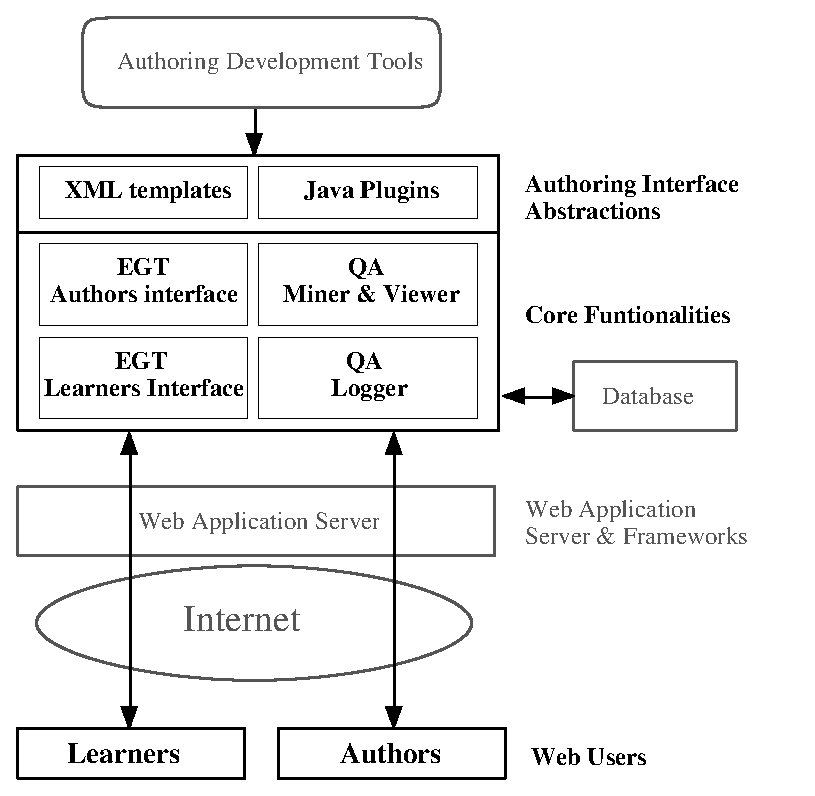
\includegraphics[width=9cm]{arch.eps}}
\caption{The LeVinQuam platform architecture overview.}
\label{arch}
\end{figure}

{\em Data input validation:}
The structure and contents of exercises, e-learning
guided tours and answers  are described in XML in the platform ({\bf EGT} blocks in the synopsis of figure \ref{arch}).
The use of a schema language for XML, as \textsc{Relax NG}, allows an
automatic validation of the exercises descriptions submitted by 
authors by matching these descriptions to an XML schema. The same
process can apply to student answers, once translated into XML in the
platform. The link between exercises and answers can also be made
explicit by means of XML syntax. Logical data input validation is a
fundamental mean for ensuring a reliable processing of these data.

%MS dans ce qui suit, on n'explique pas assez les composants de la
%figure sur l'architecture

{\em Authoring interfaces:}
The platform layer does not pretend to offer to authors an exhaustive
set of graphical-oriented authoring tools, which would represent a
full development project per se.  This is why authoring tools appear
at the top, outside the core area in  figure \ref{arch}.
In contrast we propose to bridge the gap between authors, developers
and the platform by providing an effective set of {\em authoring
interfaces} allowing them to enrich the platform with their own
extensions, letting them define new exercises types, new answers
validators, and further new graphical-oriented authoring tools to help
in these tasks.
%To provide a reliable extension framework, allowing and
%encouraging teachers and researchers to capitalize and share
%contributive developments in an effective manner, robust and open
%standards like XML and Java will be used as root technologies (even if
%rapid application development complements can be further plugged
%in). These authoring interfaces are based on concepts of {\em XML templates} and {\em java plug-ins}.

%MS la phrase pr�c�dente n'est-elle pas un peu redondante avec avant
%et... la suite?
%PD ok, vu.

In a first phase, authors, with the help of a simple
validating XML editor,  fill XML templates describing their
exercises and answers. A template library providing simple generic
types of exercises is proposed to the authors for this purpose. 
%We think
%that XML is simple enough to be quickly mastered by authors because it
%focuses on structure and contents (by contrast, HTML mixes informal
%logic and presentation style).
%Nevertheless, the
%development of authoring tools is encouraged thanks to XML playing the
%role of a common language for interfacing with the core platform.
In a second phase graphical-oriented authoring tools extensions to the
platform  propose to authors a user-friendly environment for
designing exercices and  output the necessary XML data for the
underlying platform authoring interfaces. In both cases, the platform
handles the code generation required to put the exercices on line,
whatever method has been employed by authors for their description.

%\footnote{It can also handle the XML validation
%by means of predefined schemas, like kinds of questionnaires, or, in
%the contrary, infer a schema from an unconstrained XML.}.

{\em Answer validation:}
Different levels of answer validation can be provided by the platform,
according to the nature  of exercises, from syntactic validation,
like checking whether an answer is a valid calendar date, to complex
semantic validations, going through  simple semantic validation of
closed questionnaires, e.g. checking whether 
this date is the correct answer. If the question is to solve a
mathematical equation, then a simple semantic validation can
decide whether the solution is the one expected. However if we want to
analyze and validate more complex formulas, a third level of validation is
necessary, that can only be based on software code having knowledge of the application
field.
To allow authors to provide such validation codes in a robust and
effective way a Java plug-in API is supplied by the platform ({\em Java Plug-in} block in figure \ref{arch}).
For example, in the SQL case study previously mentioned, when a student
answer is an SQL query, a Java plug-in validator would send this query to a
dedicated SQL server and analyse the server's reply (here, from the standpoint of the platform,
Java is a wrapper for SQL).
We  advocate for  the usage of Java within
LeVinQam for several reasons. One of them is the huge collection of Java source code
available on the internet. Portability is also enhanced with Java, which is
a main-stream programming language. Another reason is more
technical: the ease of maintenance, compared with scripting languages,
and the richness of web frameworks based on J2EE (e.g. the java projects at {\tt apache.org}).
%MS r�f�rences 
%% We actually plan to run our platform by means of Java
%% servlets with the support of Tomcat and build the web application with
%% help of open source frameworks, like Struts and Cocoon. These
%% technologies offer a clean architectural and functional model (called
%% Model-View-Controller) and reach a wide audience among companies.

%We previously mentionned an example with SQL and this lead us to
%another aspect of the platform: data persistence. 

{\em Data persistence:}
The last feature of the platform is data persistence. All answers as well as the log of the learner's
interaction with the platform are stored in a relational  database for further data-mining
({\em QA Logger} and {\em QA Miner~\&~Viewer} in figure \ref{arch}).
We  use  XML
transformations to map exercises, answers and guided tours to
the relational database schema.

Most of the aforementioned features, especially layers of answer
validation and data persistence, have been experimented in a first
prototype \cite{wargon01} based on Ganesha \cite{ganesha}.

%MS reference de Ganesha et de laurent Wargon
%This enables further data mining to discover new informations
%and gives some feedback to the teacher. 


%% A trail is a path among the course or the exercises which is proposed
%% to the learner. There can be predefined trails like beginner's trails
%% or advanced trails, but also unconstrained trails which allow the
%% learner to progress freely. These trails can be specified as an XML
%% schema. In all cases, the interactions of the learner along his trail
%% is recorded in the platform database for future mining.




\section{Visualisation and Mining} %AM 
\label{visualisation}
The rich information model that we adopt for our platform makes it possible to provide facilities to teachers in order to assist them in  their  pedagogical follow up of students. % This is done at two levels. 
First, it is possible to convey to teachers (part of the) information
that they implicitely have when they do face to face teaching. Second,
additional information can be provided due to the technology
change. Indeed, having all students (guided) tours, answers,  mistakes and,
possibly, teachers annotations stored and accessible in a database
makes it possible to use queries and Data mining techiques to retrieve
pedagogically relevant information for both students and
teachers~\cite{amv03}. Here, we focus on the teacher's point of view. 

We illustrate  our approach   with the Logic-ITA, which can be seen as a particular application case of our platform.

The Logic-ITA is a web-based intelligent teaching assistant system for the domain of
formal proofs in propositional logic currently in use at the Information Technologies School of the University of Sydney.
It provides an
environment where students can practice formal proofs of logic at their
own discretion, receiving step-by-step, contextualised feedback. They
can choose to create new exercises, select exercises in the exercise
database, or ask the system for one adapted to their needs. The system
stores, for each student, every step entered, along with
any mistake the student may have made and collates all this
information into a database. This makes the  information model of the
Logic-ITA quite close to the one proposed in our platform. LeVinQam
generalizes the Logic-ITA by providing a model of learning tours. 

We need to explain the structure of an exercise to make  the following
clearer, the reader may refer to \cite{logicT1} for more details. 

Exercises start with a given set of premises, i.e. a set of well-formed formulae (wff) of propositional logic, and exactly one wff, the conclusion. The task then consists of deriving the conclusion from the premises, step-by-step, using laws of equivalence and rules of inference (we will refer to both of these as rules for the rest of this paper). Figure \ref{screen} shows a screen shot of the interface. Here the student was given the first two lines (lines 0 and 1) and the conclusion at the bottom left corner, i.e. $C$. For each step, the student must fill out a new line, entered at the bottom of the screen. The student needs to do the following: 

\noindent
- enter a formula in the {\em Formula} section, \\
- choose, {\em  from a pop-up menu}, the rule used to derive this formula from one or more previous line(s) ({\em Rules}), \\
- the references of those previous lines ({\em  Line References}) and \\
- the premises the formula relies on ({\em  Premises}). 


\begin{figure}
{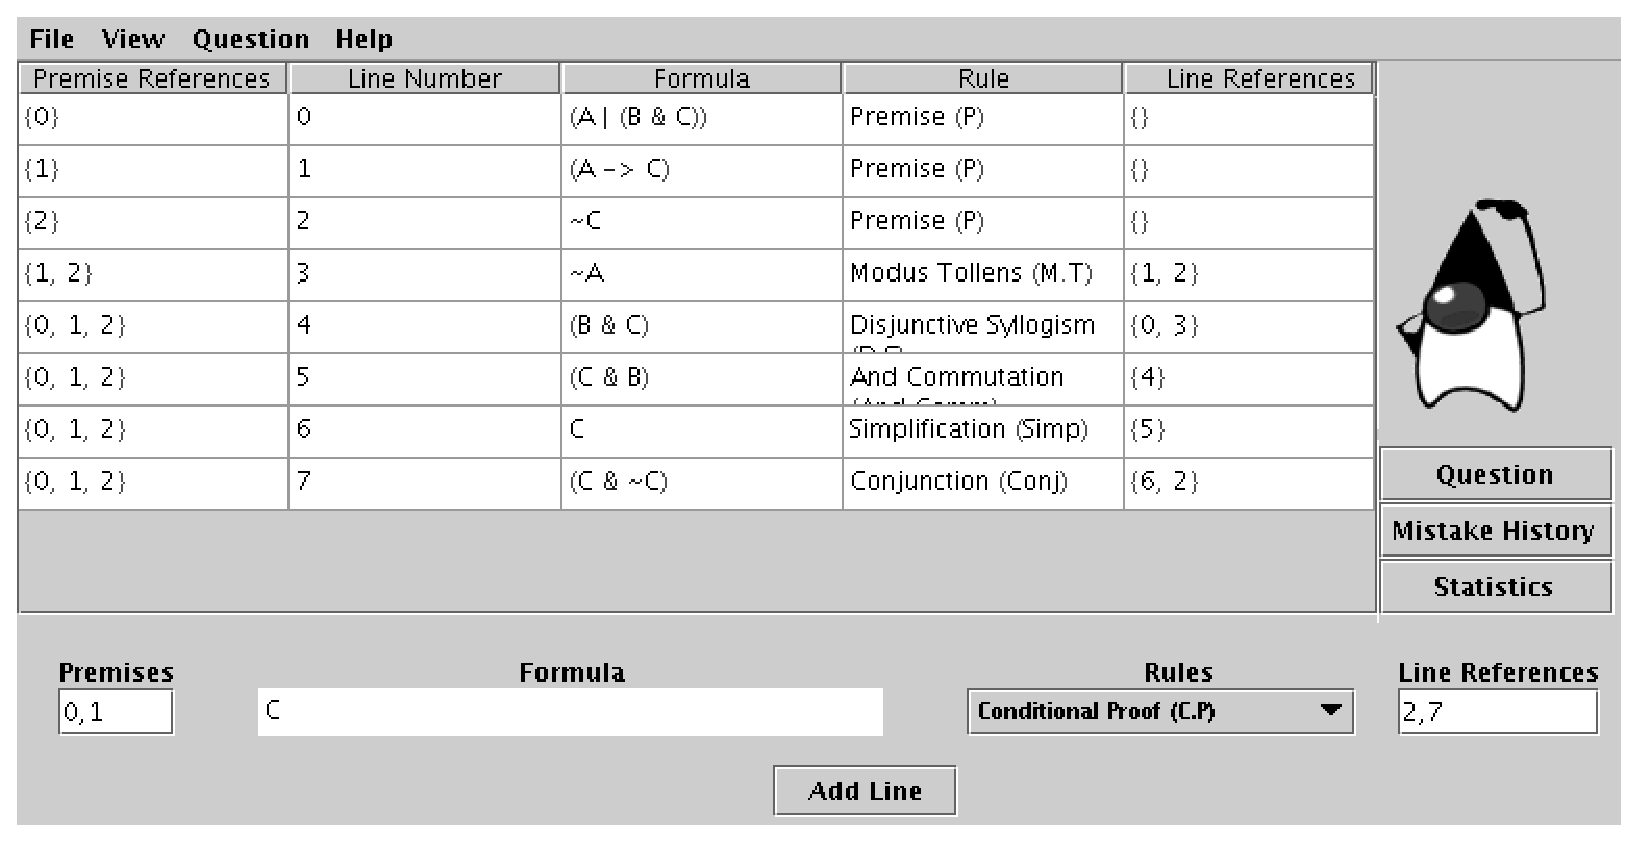
\includegraphics[width=9cm]{screenshot.eps}}
%%%\special{psfile=screenshot.ps hoffset=-15 voffset=-10}% hscale=60 vscale=60}
\caption{Screenshot during an exercise.}
\label{screen}
\end{figure}

For example in Figure \ref{screen}, the student is currently deriving the formula $C$, using the rule {\em Indirect Proof} and the formulae of lines 2 and 7. Because lines 2 and 7 rely respectively on premises {2} and {0,1,2} (as can be seen in the first column of the screen) and {\em Indirect proof} removes the premise 2, the line entered therefore relies on premises {0,1}. It is actually the last step of this exercise, deriving the conclusion. 

At each step, the system checks the validity of the data entered by the student. There are different types of mistakes, and, each of them is labelled with a meaningful title for the teacher. For example, the mistake message {\em Wrong reference lines} means that the student has not provided the right lines of reference the rule applies to. 
  

\subsection{Retrieving implicit information provided by face to face teaching}

%In a context of distance education, teachers do not have anymore the visual information that face to face teaching provides. An obvious example concerns course material. In face to face teaching, they know the course material students are supposed to have seen because it is what they have taught in their lectures. In our information model, storing trails of students through course material allows to retrieve this information.

In face to face teaching, teachers would be aware of students who succeed completing exercises and students who fail, on how students use the tool, in a thoughtful manner or just trying any possible exercise, any possible rule one after the other -- at least as far as classes are not too big.
Experiments with the Logic-ITA  indicate that this kind of information on students' behaviours can be conveyed to teachers.


The aim of the tool is to help students grasp formal proofs. In the
case students  make mistakes but finish successfully exercises,
teachers do not need to worry. Teachers need to be aware of students
not completing successfully exercises since they may have
difficulties. In order to characterize these latter students, a
 k-means clustering \cite{han} has been applied, taking
into account the recorded mistakes. The clustering  yields three
classes. Class 1 is composed of students making few mistakes, class 2
of students making an intermediate number of mistakes and class 3
students making many mistakes, see \cite{akwww04} for more details.
Then several graphs have been produced. A first graph plots {\em
logins} (i.e. student identification) against {\em exercise-id}
(exercise identification).  Thus this graph visualizes the various
exercises attempted by each student. The trend given by this graph is
that students of class 1  attempt more exercises than  students from
class 2 or 3. A second graph plots {\em logins} against {\em
mistake-messages}. The trend given by this graph is that students from
class 2 or 3 make more different kinds of mistakes that students from
class 1. Students from class 1 make the mistakes that are most usually
made by everybody using the tool.  Plotting {\em logins} against {\em
logical-rules} used in the non-completed exercises gave the graph
given in Figure \ref{loginRules}. This graph shows vertical lines for
several students from  class 2 or 3 only, not from class 1. Students
from class 1 constitute the narrow green strip in the middle of the
graph. A vertical line means that all rules have been tried while
doing the exercises.  They suggest that these students have just tried
one rule after the other from the pop-up menu, apparently adopting a
behaviour of "guess and test" strategy. Awareness of these behaviours
may lead teachers to differentiate their pedagogy. 

\begin{figure}[htbp]
{\includegraphics[width=9cm]{login_rule2.eps}}
%% \special{psfile=LoginRule2.ps hoffset=-15 voffset=-10}% hscale=60 vscale=60}
\caption{Plot of Students against Logic Rules.}
\label{loginRules}
\end{figure}


\subsection{Extracting hidden information}

Using Data Mining techniques on students'answers stored in the database can lead to discover  patterns that quite often remain hidden or not well defined otherwise. We have used the association rule algorithm to all the answers from the Logic-ITA to be aware of mistakes often made together while solving exercises. Figure \ref{diagnosis} shows parts of the result, \cite{AK-AIeD} gives more details. 

As an example, the association
{\em Rule can be applied, but deduction incorrect} $\rightarrow $
{\em Premise set incorrect} means that while solving an exercise, if a student makes the mistake {\em Rule can be applied, but deduction incorrect} then s/he makes also the mistake {\em Premise set incorrect}, this association has a support of 60\%. and a confidence of 82\%.
Support makes sure that only mistakes occurring
often enough in the data will be taken into account. Confidence is a measure of how much  $Y$  is really
implied by $X$ in the rule  $X$ $\rightarrow $ $Y$.  


First, we  explain what these mistake messages mean, refering to the example
shown in Figure \ref{screen}. Consider
line 3. If the student  gives
the formula $A$ instead of $~A$, the mistake 
{\em Rule can be applied, but deduction incorrect}
is made.
Indeed, {\em Disjunctive Syllogism} can be applied, but the negated left side of the formula given line 1 can be deduced, as shown in Figure \ref{screen}, not the positive form as written here.  Suppose now that the student gives only 1
in the $Prem.$ field. Then the mistake {\em Premise set incorrect}
is made.
Finally, suppose that the student  gives only 1 in the $Re\!f\!s.$
field. Then a 
{\em Wrong number of line references given} mistake is
 made, because 2 lines of reference are needed.

  
\begin{figure}
\begin{tabular}{|l|c|c|}
\hline
association & supp. & conf.\\
\hline
{\em Rule can be applied, but deduction incorrect} & \ & \ \\
 $\rightarrow $
{\em Premise set incorrect} & 61\% & 82\%\\
\ & \  & \  \\
{\em Premise set incorrect}  & \ & \ \\ 
$\rightarrow $ 
{\em Wrong number of line references given} & 67\% & 87\%\\
\ & \  & \  \\
{\em Rule can be applied, but deduction incorrect}  & \ & \ \\
$\rightarrow $  {\em Wrong number of line references given} & 65\% & 87\%\\
%{\em Premise set incorrect} $\rightarrow $
%{\em Wrong number of line references given}, & \  & \ \\
%{\em Rule can be applied, but deduction incorrect} & 0.56 & 0.73\\
%{\em Rule can be applied, but deduction incorrect},
%{\em Premise set incorrect}& \  & \ \\
%$\rightarrow $
%{\em Wrong number of line references given}& 0.56 &  0.92\\
\hline
\end{tabular}
\caption{Associations found focusing on mistake messages.}
\label{diagnosis}
\end{figure}

The associations found  show relations between
mistakes involving line numbers in the premises
({\em Premise set incorrect}), 
  line numbers in the reference lines a logic rule 
applies to ({\em Wrong number of line references given})
and  incorrect use
 of logic rules ({\em Rule can be applied, but deduction incorrect}).
This confirms what human tutors had sensed.
First, students often have difficulties at grasping
all details required in a proof: one has to provide
not only a logic rule, but also the lines it applies to,
and these are different from the premises involved.
Second, students do not realize at once that there
are two kinds of logic rules:  rules of equivalence that
are applied to one formula only, and  rules of inference
that are mostly applied to two formulas.
Most importantly, rules of
equivalence can be applied to subparts of a formula whereas rules of
inference can only be applied to whole formulae. For example in the
formula $((A \wedge  B) -> C)$ we can validly replace $(A \wedge B)$
 with $(B \wedge A)$ in the formula 
using the rule of equivalence {\em And Commutation} but it is not valid
to deduce $B$ from  $((A \rightarrow B) \rightarrow C)$ and $A$
 using the
rule of inference {\em Modus Ponens}.
Following these findings, presentation of the course material has been revised to put more emphasis on the differences between rules of equivalence
and rules of inference.  



%\section{Case studies} %AM 
%\label{caseS}
%\input{caseS.tex}

%\section{Conclusion} % 
%\label{concl}
%%%-*-latex-*-

\section{Conclusion\label{conclusion}}

In this paper we have presented a global test architecture for  
distributed services including the generation of test sequences for
service components. Our approach was validated by a case study: a
France Telecom \audio service.

The full service was described using the SDL language, and the running
of the Hit-or-Jump algorithm showed no deadlocks and produced the test
sequences for all the components of the studied service.

For sake of simplicity, we have selected a component of the \audio service
that is at the very heart of the service, the conference bridge, and
which coordinates the other components and illustrates clearly what
one imagines a \audio service is. The other components were generic
components that can be present in other kind of telecommunication
services, and for which we also generated the corresponding tests. We
have produced the tests for the bridge component in its context, and
we translated them in the TTCN and MSC formats.

We have also defined an architecture for the tester, which combines an
active part (based on a stimulation of the implementation) and a
passive one (based on the observation of the exchanges between the
CORBA objects). 

The results we got show that the use of formal methods considerably
eases the task of the service designers and developers, and that they
are usable for real services. Since the design phase to the
implementation and test phases, we used formal description techniques
(SDL, TTCN, MSC) and a formal test methodology. Moreover, we showed it
is possible to test the service components in the context of the
others (and not artificially in isolation). We think this is a notable
step towards the validation and the design of reusable
service-components.



\begin{thebibliography}{12}
% Note the sample label "11" in thebibliography
% This is like the new IEEEtran class'
% \begin{enumerate}[\setlabelwidth{11}]


%\end{thebibliography}
\bibitem{logicT1}
D.~Abraham, L.~Crawford, L.~Lesta, A.~Merceron  and K.~Yacef,
``The Logic Tutor: A Multimedia Presentation'', {\em Interactive 
Multimedia Electronic Journal of Computer-Enhanced learning}, Vol.~3, 
Nb.~2, Nov. 2001.



\bibitem{amv03} B. Aguado, A. Merceron and A. Voisard, ``Extracting
Information from Structured Exercises'',  Proceedings of  the 4th
International Conference on Information Technology Based Higher
Education and Training ITHET03, Marrakech, Morocco, (2003).

\bibitem{akwww04}
Benchaffai M., Debord G., Merceron A., and Yacef K., {\it TADA-Ed, a tool to visualize and mine students' work}. Submitted paper. 2004

%\bibitem{duboulay01} B.~du Boulay, R.~Luckin, ``Modeling Human
%Teaching Tactics and Strategies for Tutoring Systems,'' {\em
%International Journal of Artificial Intelligence in Education,}
%Vol.~12, pp. 235-256, 2001

\bibitem{Brusilovsky} P.~Brusilovsky, ``Adaptive and Intelligent
Technologies for Web-based Education'' {\em K\"unstliche Intelligenz,
Special Issue on Intelligent Systems and Teleteaching,  4, 19-25, 1999

%\bibitem{Laos}
%A.I.~Cristea and A.~de~Mooij,
%``LAOS: Layered WWW AHS Authoring Model and their corresponding 
Algebraic Operators'',
%{\em Proceedings of the track Education, 12th International World Wide 
Web Conference WWW2003}, www2003.org, Budapest, Hungary, pp.185-194, May 
2003

%\bibitem{druger00}
%M.~Druger, ``A Perspective on Exams and Grading'', {\em Journal
%of College Science and Teaching''}, Vol.~30, Issue~3, pp. 210-211,
%2000.

%\bibitem{ellard02}
%C.~Ellard, M.~Feinberg, J.~S. Siekpe, ``Classifying student errors
%in the introduction to microeconomics course,'' {\em Business Quest,
%Journal of Applied Topics in Business and Economics}, 2002.

\bibitem{wargon01}
Laurent Wargon, ``Une plateforme d'apprentissage de SQL en ligne'', {\em Rapport interne},
ESILV/GI, January 2004.

\bibitem{ganesha}
http://www.anemalab.org/ganesha/,
Ganesha, a Learning Management System

\bibitem{grandbastien03}
M.~Grandbastien, L.~Oubahssi, G.~Claes, ``A process oriented approach 
for modelling on line Learning Environments'', {\em Supplementary 
Proceedings of Artificial Intelligence in Eudcation AIED2003}, 
University of Sydney, Australia, pp.~140-152, July 2003.


\bibitem{han}
Han J.,  and Kamber M.,
{\it Data Mining: Concepts and Techniques},
Morgan Kaufmann Publishers, 2001


\bibitem{Petri}
K. Jensen ``An Introduction to the Theoretical Aspects of Coloured Petri Nets.'' {\em A Decade of Concurrency}, J.W. de Bakker, W.-P. de Roever, G. Rozenberg (eds.), Lecture Notes in Computer
Science vol. 803, Springer-Verlag, 230-272, 1994

%\bibitem{jean00}
%S.~Jean, {\em Ppite: un syst\`eme d'assistance au diagnostic de
%comp\'etences}.
%\newblock Ph.D.\ thesis, University of Le Mans, France, 2000.

%\bibitem{langley84}
%P.~Langley, S.~Ohlsson, ``Automated Cognitive Modeling,''
%{\em Proceedings of the Second National Conference on Artificial
%Intelligence}, 1984.



%\bibitem{leroux96}
%O.~Leroux, M.~Vivet, P.~Brezillon, ``Cooperation between a Pedagogical
%Assistant, a Group of Learners and a Teacher,''
%{\em Proceedings of European Conference on AI in Education},
%Lisbon, Portugal, pp.~379-385, 1996



\bibitem{AK-AIeD}
A.~Merceron  and K.~Yacef, ``
A Web-Based Tutoring Tool with Mining
Facilities to Improve Learning and Teaching'',
{\em Proceedings of the 11th International Conference
on Artificial Intelligence in Education}, Sydney, Australia, pp.201-208, 2003

%\bibitem{SmartSpace}
%B.~Simon, Z.~Miklos, W.~Neidl, M.~Sintek and J.~Salvachua,
%``Smart Space ofr Learning: A Mediation Infrastructure for Learning 
%Services'',
%{\em Proceedings of the track Education, 12th International World Wide 
%Web Conference WWW2003},  www2003.org, Budapest, Hungary, pp. 97-101, 
%May 2003


\end{thebibliography}












\end{document}

% END of IEEEtest.tex ************



-----------------------------7d34613d68--
